\chapter{Analysis}

\section{Datasets}
In the context of this research, I have been granted access to two distinct generated datasets, produced utilizing SNIPER, a leading-edge simulation tool deployed within the framework of the JUNO experiment. 

The first of the datasets provided is specifically tailored for the study of Inverse Beta Decay (IBD) events. Each event within this dataset, simulated and injected into the system, is tagged with a unique Simulation Identifier, or SimID. Furthermore, events which trigger a sufficient number of PMTs to be captured by the electronic system are assigned an EventID. This intricate labeling system allows for a clear differentiation between correlated IBD events, which represent actual IBD occurrences, and uncorrelated IBD events.



The second dataset focuses primarily on radioactivity events. Similar to the IBD dataset, it encompasses a large number of simulated events, each reflecting the complex reality of real-world physics phenomena. Additionally, the inherent electronic noise prevalent in actual physical environments is accurately accounted for, ensuring a realistic representation within the simulated context.

In this research undertaking, my central task will focus on a detailed examination and evaluation of the provided datasets. My work will primarily involve not just interpreting the inherent characteristics and peculiarities of the recorded events, but also harnessing these insights to construct comprehensive feature tables. These feature tables, generated from the datasets, will serve as the basis for my subsequent analysis and interpretation, a process which will be elaborated upon in the following sections of this study. The aim is to provide a meaningful understanding of the correlations and implications of these events within the broader context of the JUNO experiment.
%TODO-> Inserire il fatto che i dataset sono stati creati in ordine temporale in parallelo con SimID Per simulare 1500000 eventi nel MonteCarlo ci vorrebbero mesi e mesi di tempo macchina.
Per affrontare il problema, si parallelizza la simulazione su una infrastruttura chiamata DCI (Distributed Computing Infrastructure).
In questo modo si può ad esempio dividere i 1500000 eventi in 1500 jobs (simulati quindi da 1500 CPU diverse) da 1000 event ciascuno, completando la produzione in poche ore invece che in mesi.
Questo approccio ha però il drawback che ogni simulazione parallela sarà indipendente dalle altre e quindi per ciascuna di queste il tempo, i SimID e tutte le altre quantità partirano da 0"" 

%La seconda colonna -> Si, sono il numero di eventi generati. Non tutti gli eventi generati interagiscono con il detector: un evento generato nella struttura metallica può venire fermato nella struttura stessa e non interagire con il detector, o ancora un evento generato nell'acrilico può venire emesso verso l'esterno e quindi non entrare mai in contatto con il detector e così via.
%Se consideri ora solo gli eventi che davvero sono entrati in contatto con il detector, non tutti gli eventi vengono ricostruiti: alcuni eventi sono così poco energetici che non sono sufficienti ad illuminare i PMT e quindi ad azionare il trigger per l'acquisizione dell'evento.

%Per darti un'idea, la rate di decadimenti radioattivi è circa 6.6 MHz, ne vengono effettivamente registrati dal detector appena 100 Hz (o poco meno)

%Questa è una delle sfide più grandi, perchè devi portare un segnale di circa 100 Hz (8.6 x 10e6 eventi/giorno) a rappresentare meno di 1 evento/giorno di background
%-------------------

%Nel MonteCarlo sono inclusi tutti gli effetti che ci aspettiamo nella realtà. E purtroppo, nella realtà, l'elettronica ha un rumore intrinseco (ad esempio puoi cercare in letteratura il Dark Count Rate per i PMTs).
%Ora, nel MonteCarlo vengono iniettati degli eventi (ad esempio una coppia prompt-delayed da IBD). A questo evento iniettato viene associato un SimID (simulation identifier) incrementale. Siccome prompt e delayed sono stati iniettati assieme, avranno lo stesso SimID.
%Non tutti gli eventi però sono registrati e salvati dall'elettronica. In JUNO, un evento viene salvato solo se questo è in grado di illuminare nello stesso momento un gran numero di PMTs (corrispondenti a qualche centinaio di keV).
%Se questo avviene, viene generato un trigger, viene salvato l'evento e gli viene associato un EventID incrementale.
%Può succedere che, per puro caso, il rumore intrinseco dell'elettronica "accenda" nello stesso momento un gran numero di PMT. In questo caso, nessun evento vero di fisica ha generato questo trigger, ma l'elettronica acquisisce e salva comunque questo evento, perch`ha superato la soglia di trigger. Quello che succede in questo caso è che l'evento avrà un EventID, ma nessun SimID associato, perchè nessun evento è stato davvero iniettato nella simulazione.
%Al contrario, può succedere che tu inietti una certa particella a cui quindi viene associato un SimID), ma questa non riesce a illuminare abbastanza PMT, l'evento non viene salvato e quindi non gli viene associato nessun EventID e non viene salvato nel file finale.


%Prima coppia simulata si becca SimID di 0. Gli Event IDs associati saranno 0 e 1.
%Seconda coppia generata avrà SimID di 1. EventIDs in questo caso sarnno 2 e 3. Ecc ecc.
%Sono incrementali per convenzione.

%TODO-> Spiega cosa c'è nei datasets -- ['EventID', 'SimID', 'timestamp', 't_sec', 't_nanosec', 'recx', 'recy', 'recz', 'm_QEn', 'm_pe']
%TODO-> Mention unbalanced datasets problem


Ciao Fabio, la radioattività con cui hai lavorato rappresenta tutto il contributo da decadimenti radioattivi (alfa, beta, gamma) interno ed esterno a detector, ma che hanno depositato energia all'interno del detector.
Ti lascio la tabella degli isotopi e delle rate di decadimento generate qui di seguito:


| **Dataset Name**  | **Number of Events**  | **Rates (used in elecsim)**  |
|:----------------: |:--------------------: |:---------------------------: |
|      U238@LS      |   1,000,000 events    |           3.234 Hz           |
|     Th232@LS      |   1,000,000 events    |           0.733 Hz           |
|      K40@LS       |   1,000,000 events    |           0.53 Hz            |
|     Pb210@LS      |   1,000,000 events    |           17.04 Hz           |
|      C14@LS       | 1,000,000,000 events  |           3.3e4 Hz           |
|      Kr85@LS      |   1,000,000 events    |           1.163 Hz           |
|   U238@Acrylic    |   10,000,000 events   |           98.41 Hz           |
|   Th232@Acrylic   |   10,000,000 events   |           22.29 Hz           |
|    K40@Acrylic    |   10,000,000 events   |          161.25 Hz           |
|   U238@node/bar   |  100,000,000 events   |          2102.36 Hz          |
|  Th232@node/bar   |  100,000,000 events   |          1428.57 Hz          |
|   K40@node/bar    |  100,000,000 events   |           344.5 Hz           |
|   Co60@node/bar   |  100,000,000 events   |           97.5 Hz            |
|   U238@PMTGlass   | 1,000,000,000 events  |          4.90e6 Hz           |
|  Th232@PMTGlass   | 1,000,000,000 events  |          8.64e5 Hz           |
|   K40@PMTGlass    | 1,000,000,000 events  |          4.44e5 Hz           |
|  Tl208@PMTGlass   | 1,000,000,000 events  |          1.39e5 Hz           |
|    Co60@Truss     |           0           |             ? Hz             |
|    Tl208@Truss    |           0           |             ? Hz             |
| Rn222@WaterRadon  |  100,000,000 events   |            90 Hz             |


\section{Feature creation}
The development of machine learning models for the detection of Inverse Beta Decay (IBD) events necessitates a systematic and efficient approach to feature engineering. This process begins with the loading of two separate datasets, one for IBDs and one for radioactivity background, each containing a multitude of potential IBD events. The primary objective is to construct a feature table that encapsulates the unique characteristics of these events, providing a robust foundation for subsequent model training.

\subsection{IBD dataset}
As we mentioned earlier, an IBD event is characterized by two distinct signals with different energies, positions, and times. The first, known as the prompt signal, is caused by the annihilation of a positron with an electron in the scintillator liquid. This interaction yields a signal with a characteristic energy. The second, the delayed signal, results from the capture of a neutron by the scintillator liquid. This signal occurs with a significant delay, at a different position, and with a different energy compared to the prompt signal.

To create the feature table, all possible pairs of events within the dataset were considered, without repetition. Each possible combination was ordered temporally, meaning the second event followed the first. This temporal ordering is crucial in feature determination. Given a pair $i-j$, and considering that neutron capture occurs temporally subsequent to electron-positron annihilation, the following features were constructed:


\begin{itemize}
	 
	\item \textbf{$R_{prompt}$}: This feature represents the distance of the prompt signal, calculated as the distance from the origin to the point $(x_i, y_i, z_i)$ in the detector space where the prompt signal occurred.	
	
	\item $R_{delayed}$: Similar to $R_{prompt}$, this feature represents the distance of the delayed signal, calculated as the distance from the origin to the point $(x_j, y_j, z_j)$ in the detector space where the delayed signal occurred.

	\item \textbf{$E_{prompt}$}: This feature represents the energy of the prompt signal. It captures the characteristic energy released during the annihilation of a positron with an electron in the scintillator liquid.

	\item \textbf{$E_{delayed}$}: This feature represents the energy of the delayed signal. It captures the energy released when a neutron is captured by the scintillator liquid. This capture can occur by hydrogen, resulting in a gamma ray with an energy of approximately 2.2 MeV, or by carbon, resulting in gamma rays with combined energies of about 4.95 MeV to 5.12 MeV.

	\item \textbf{$\Delta_{Time}$}: This feature represents the time difference between the two events. It captures the temporal delay between the occurrence of the prompt and delayed signals.

	\item \textbf{$\Delta_{Radius}$}: This feature represents the spatial distance between the two events. It captures the spatial separation between the points in the detector space where the prompt and delayed signals occurred.

\end{itemize}
These features encapsulate the temporal and spatial differences between the prompt and delayed signals, as well as their respective energies, providing a comprehensive representation of the unique characteristics of IBD events.


\subsubsection*{Event Labeling}

In the context of supervised learning, the process of labeling is crucial as it provides the ground truth against which the performance of the machine learning model is evaluated. In this scenario, each pair of events in the dataset is assigned a label that indicates whether it represents a true Inverse Beta Decay (IBD) event or a background signal (BKG).

The label is a binary value: a label of 1 signifies a true IBD event, while a label of 0 signifies a BKG event. The assignment of these labels is not arbitrary but is guided by a specific criterion based on the simulation identifier (SimID) associated with each event pair.

The SimID is a unique identifier assigned to each simulated event pair during the generation of the dataset. If a pair of events share the same SimID, it means they were generated as part of the same simulation and thus are considered to represent a true IBD event. In this case, they are assigned a label of 1.

Conversely, if a pair of events do not share the same SimID, it means they were generated as part of different simulations. These events are not correlated and thus are considered to represent BKG events. In this case, they are assigned a label of 0.

This labeling strategy based on the SimID ensures a systematic and consistent methodology for event classification. It provides a clear and objective criterion to distinguish between true IBD events and BKG events, which is essential for the training and evaluation of the machine learning model.


\subsubsection*{Efficient Feature Calculation}
Given the large size of the dataset and the computational complexity of feature calculation, a parallel computing approach was adopted to enhance efficiency. The feature calculation task was divided into multiple sub-tasks that could be executed simultaneously by different cores of a CPU. This parallelization significantly reduced the total computation time, particularly beneficial when working with large volumes of data.


To further optimize the computation, a method was implemented to only consider event pairs where the delayed event occurs within a time window of $5*\tau$ from the prompt event. This approach is based on the fact that the time delay between the prompt and delayed events in Inverse Beta Decay (IBD) typically follows an exponential distribution, a characteristic of radioactive decay processes. While this method significantly reduces the number of potential event pairs, it might exclude about $0.7\%$ of IBD events that occur outside this time window. 

While this percentage is relatively small, it's important to consider the potential impact on the analysis results.

\subsection{Radioactivity dataset}
For the radioactivity dataset, the feature calculation was performed in a manner analogous to the IBD dataset. The key difference is that event pairs from the radioactivity dataset are labeled as BKG events, hence assigned a label of 0.



\begin{figure}[h]
	\centering
	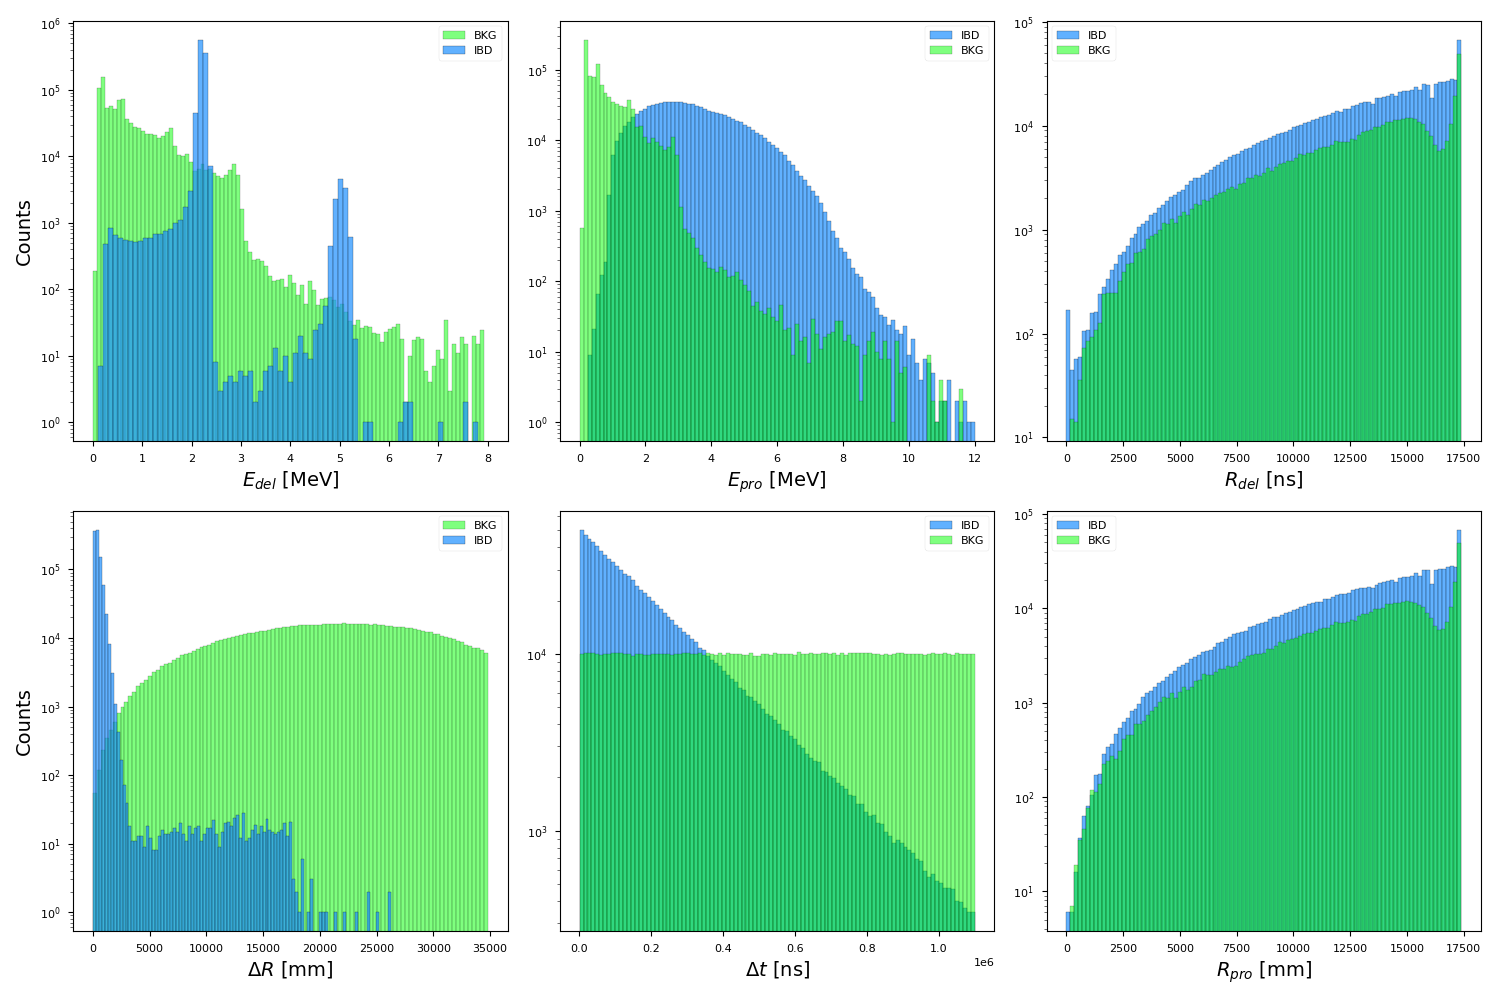
\includegraphics[width=1\linewidth]{Images/hist_features.png}
	\caption{Features histograms}
	\label{fig:hist_features}
\end{figure}



In summary, the feature engineering process for IBD event detection involves careful consideration of the unique characteristics of these events, systematic feature construction, and efficient computation strategies. This process provides a robust foundation for the development and training of machine learning models for IBD event detection.

\section{Models}
\subsection{Manual Cut}
\subsection{XGBoost}
\subsection{PyThorch}

\section{Conclusion}

% Please add the following required packages to your document preamble:
% \usepackage[table,xcdraw]{xcolor}
% If you use beamer only pass "xcolor=table" option, i.e. \documentclass[xcolor=table]{beamer}
\begin{table}[h!]
	\begin{tabular}{lllll}
		\cline{1-3}
		\multicolumn{1}{|l|}{} & \multicolumn{1}{c|}{{\color[HTML]{CE6301} \textbf{Manual Cut Algorithm}}} & \multicolumn{1}{l|}{{\color[HTML]{009901} \textbf{BDT Algorithm}}} &  &  \\ \cline{1-3}
		\multicolumn{1}{|l|}{\textit{Radioactivity}} & \multicolumn{1}{l|}{\begin{tabular}[c]{@{}l@{}}Efficiency: 99.9973\%\\ Purity: 100\%\end{tabular}} & \multicolumn{1}{l|}{\begin{tabular}[c]{@{}l@{}}Efficiency: 99.997684\%\\ Purity: 100\%\end{tabular}} &  &  \\ \cline{1-3}
		\multicolumn{1}{|l|}{\textit{True IBDs}} & \multicolumn{1}{l|}{\begin{tabular}[c]{@{}l@{}}Efficiency: 97.734\%\\ Purity:100\%\end{tabular}} & \multicolumn{1}{l|}{\begin{tabular}[c]{@{}l@{}}Efficiency: 99.997616\%\\ Purity: 100\%\end{tabular}} &  &  \\ \cline{1-3}
		&  &  &  & 
	\end{tabular}
\end{table}

